% !TEX TS-program = pdflatex
% !TEX encoding = UTF-8 Unicode

% This is a simple template for a LaTeX document using the "article" class.
% See "book", "report", "letter" for other types of document.

\documentclass[journal, a4paper]{article} % use larger type; default would be 10pt

\usepackage[utf8]{inputenc} % set input encoding (not needed with XeLaTeX)

%%% Examples of Article customizations
% These packages are optional, depending whether you want the features they provide.
% See the LaTeX Companion or other references for full information.

%%% PAGE DIMENSIONS
\usepackage{geometry} % to change the page dimensions
\geometry{a4paper} % or letterpaper (US) or a5paper or....
% \geometry{margin=2in} % for example, change the margins to 2 inches all round
% \geometry{landscape} % set up the page for landscape
%   read geometry.pdf for detailed page layout information

\usepackage{graphicx} % support the \includegraphics command and options

% \usepackage[parfill]{parskip} % Activate to begin paragraphs with an empty line rather than an indent

%%% PACKAGES
\usepackage{booktabs} % for much better looking tables
\usepackage{array} % for better arrays (eg matrices) in maths
\usepackage{paralist} % very flexible & customisable lists (eg. enumerate/itemize, etc.)
\usepackage{verbatim} % adds environment for commenting out blocks of text & for better verbatim
\usepackage{subfig} % make it possible to include more than one captioned figure/table in a single float
% These packages are all incorporated in the memoir class to one degree or another...

%%% HEADERS & FOOTERS
\usepackage{fancyhdr} % This should be set AFTER setting up the page geometry
\pagestyle{fancy} % options: empty , plain , fancy
\renewcommand{\headrulewidth}{0pt} % customise the layout...
\lhead{}\chead{}\rhead{}
\lfoot{}\cfoot{\thepage}\rfoot{}

%%% SECTION TITLE APPEARANCE
\usepackage{sectsty}
\allsectionsfont{\sffamily\mdseries\upshape} % (See the fntguide.pdf for font help)
% (This matches ConTeXt defaults)

%%% ToC (table of contents) APPEARANCE
\usepackage[nottoc,notlof,notlot]{tocbibind} % Put the bibliography in the ToC
\usepackage[titles,subfigure]{tocloft} % Alter the style of the Table of Contents
\usepackage{float}
\usepackage[colorlinks = true,
            linkcolor = blue,
            urlcolor  = blue,
            citecolor = blue,
            anchorcolor = blue]{hyperref}
\usepackage{url}
\usepackage{graphicx}
\usepackage{mhchem}
\usepackage{amsmath}
\usepackage{amssymb}
\usepackage{multicol}
\usepackage{microtype}    
\graphicspath{{Figures/}}
\renewcommand{\cftsecfont}{\rmfamily\mdseries\upshape}
\renewcommand{\cftsecpagefont}{\rmfamily\mdseries\upshape} % No bold!

%%% END Article customizations

%%% The "real" document content comes below...

\title{Summary of Redfish 2013}
\author{}
%\date{} % Activate to display a given date or no date (if empty),
         % otherwise the current date is printed 


\begin{document}


%\maketitle
%\begin{multicols}{2}
%\newpage
\section{Project}

The project, \textit{Carbon and Nutrient Draw-down in the Surface Layer of the Irminger and Labrador Seas}, is the first phase of a long-term study. Researchers examined carbon and nutrient data from the Irminger Sea and the Labrador Sea. Samples were taken in the upper 100m of the water column. Two cruises, RFI and RFG, took place during the late spring and early summer of 2013. RFI sampled the Irminger Sea and RFG sampled the Labrador Sea. Parameters of interest included the carbonate system and macronutrients. Chlorophyll imagery was used to enhance the results of the cruises. 
 

\section{Objective}


The main objective of Redfish 2013 was to examine inorganic carbon and nutrient dynamics in the Irminger Sea and nearby waters. Researchers involved in the project hoped to establish a baseline for future testing in the study region.


 
\section{This document}



The Redfish 2013 project was abandoned and this document was written in an effort to assemble and reorganize the data. Below is a file guide and summary of the results of the Redfish 2013 data. The student responsible for the Redfish project, Ryan Barkhouse, left no file guide for any of his work. As a result, some of his data, methods, and motivations can only be speculated. 
\\[12pt]
The files have been separated for the sake of cleanliness and organization. The outdated/original files are at \path{/redfish_project/old_barkhouse_files}, while the newer files are at \path{/redfish_project/redfish}. Within these two folders are a number of different files and folders that are explained below. 
\newpage
\section{Guide for the updated directory}

The updated directory is at \path{/redfish_project/redfish}. There are a number of different folders within this directory. 

\subsection{Data}

Within this folder we see two files: (1) the cruise tracks from Redfish 2013 and (2) the 2013 data.
\\[12pt]
(1) The cruise tracks were produced in ODV and are a simple snapshot of where the project took place. 
\\[12pt]
(2) These are the measurements from Redfish 2013. There is a lot of data from the project. The sources for the data in this spreadsheet are listed in Table \ref{t:RFIsources} and Table \ref{t:RFGsources} in the appendix. The parameters/variables listed in these tables are limited to those that are relevant to the project's objective. 

\subsection{File guide}

Self-explanatory.  

\subsection{LDEO database}
Updated LDEO database (Version 2017). The LDEO data is not relevant to the project. However, since Barkhouse had an older version of the dataset in his files we have chosen to include an updated database.  

\subsection{R code}
R code used to analyze the data from the 2013 data. 

\section{Guide for the outdated directory} 

The outdated directory is at \path{/redfish_project/old_barkhouse_files/Redfish 2013}. 

\subsection{Papers}

There are two folders in this directory that contain papers. One holds a paper Barkhouse was working on as well as his thesis (\path{/redfish_project/old_barkhouse_files\Redfish 2013/Barkhouse_Papers}). The other holds literature that was relevant to his work (\path{/redfish_project/old_barkhouse_files/Redfish 2013/Relevant_Papers}). 

\subsection{LDEO and CARINA}
Barkhouse was combining Redfish 2013 data with the LDEO and CARINA datasets. The work done in some of his Excel spreadsheets suggests that he was interested in long-term pCO2 trends in the North Atlantic. However, the trends do not appear to be statistically significant. Therefore, both the LDEO and CARINA datasets and folders/files are considered to be irrelevant to the objective of the project. 
\\[12pt]
The most important data from either of these folders is within \path{CARINA_COMBINED.xls}. The pCO2 spreadsheet in this file is the source for the pCO2 measurements in the 2013 dataset.  

\subsection{German}

The German files are the source for the RFG data in the 2013 dataset. This data is from the German cruise that participated in Redfish 2013. 

\subsection{Raw data}

This is the original Redfish 2013 dataset. This spreadsheet has been edited for clarity and is now in the updated directory. As previously mentioned, the sources for the data are listed in Table \ref{t:RFIsources} and Table \ref{t:RFGsources} in the appendix. The parameters listed in these tables are limited to those that are relevant to the project's objective. 
\\[12pt]
\noindent If you scroll horizontally on the master sheet you will find variables that we have not sourced. We have omitted this data for two reasons: (1) their source is unknown and (2) they seem to be irrelevant to the objective. 

\section{Data and results}

Results from Barkhouse's work have been recreated. To find the relevant code please refer to the updated directory. 
\subsection{Measurement Ranges}
The following measurements can be found in Table \ref{t:Ranges}. 
\\[12pt]
Nitrogen and phosphate were lowest at the surface, ranging from 0.62 – 11.84 $\mu$ mol kg$^{-1}$ and 0.17 – 0.78 $\mu$ mol kg$^{-1}$ respectively. The concentration of N and P increased with depth, reaching a range of 10.32 – 16.95 $\mu$ mol kg$^{-1}$ and 0.83 – 1.24 $\mu$ mol kg$^{-1}$ respectively at 100 m. 
\\[12pt]
pCO2 and TIC were also lowest in surface waters, ranging from 241.0 – 387.1 $\mu$atm and 2013.4 – 2142.20 $\mu$ mol kg$^{-1}$ respectively. Both pCO2 and TIC increased with depth, reaching a range of 294.8 – 417.7 $\mu$atm and 2102.4 – 2178.3 $\mu$ mol kg$^{-1}$ respectively, at 100 m. 
\\[12pt]
pH decreased with depth from between 8.03 and 8.21 at the surface to between 7.97 and 8.06 at 100 m. Alkalinity was between 2194.02 and 2329.74 at the surface and 2288.17 and 2331.28 at 100m. 
%\\[12pt]
%The highest surface concentrations of N+N, P, TIC, and pCO2 were observed in the Northwestern Irminger Sea, and the lowest were observed off the Southwest coast of Greenland.
%\\[12pt]


\subsection{Redfield drawdown}

Part of the motivation for this project was to examine the drawdown ratios of C:N:P. The observsed ratios were expected to be in close agreement with the Redfield ratio of 106:16:1.
\\[12pt]
Project data suggests good agreement with the Redfield ratio (Table \ref{t:Broad}; Figure \ref{f:redfield}). However, changing the scale affects this agreement. 
\\[12pt]
On the basin wide scale, C, N, and P drawdown ratios were close to Redfield in the Irminger Sea (Table \ref{t:RFI}). This was not the case in adjacent waters. Measurements in the Labroador Sea are relatively low compared to the Redfield ratio (Table \ref{t:RFG}). On a more localized scale there was wide variation in the drawdown ratios of C, N, and P from station to station. 
\\[12pt]
\begin{figure}[htbp]
	\begin{center}
		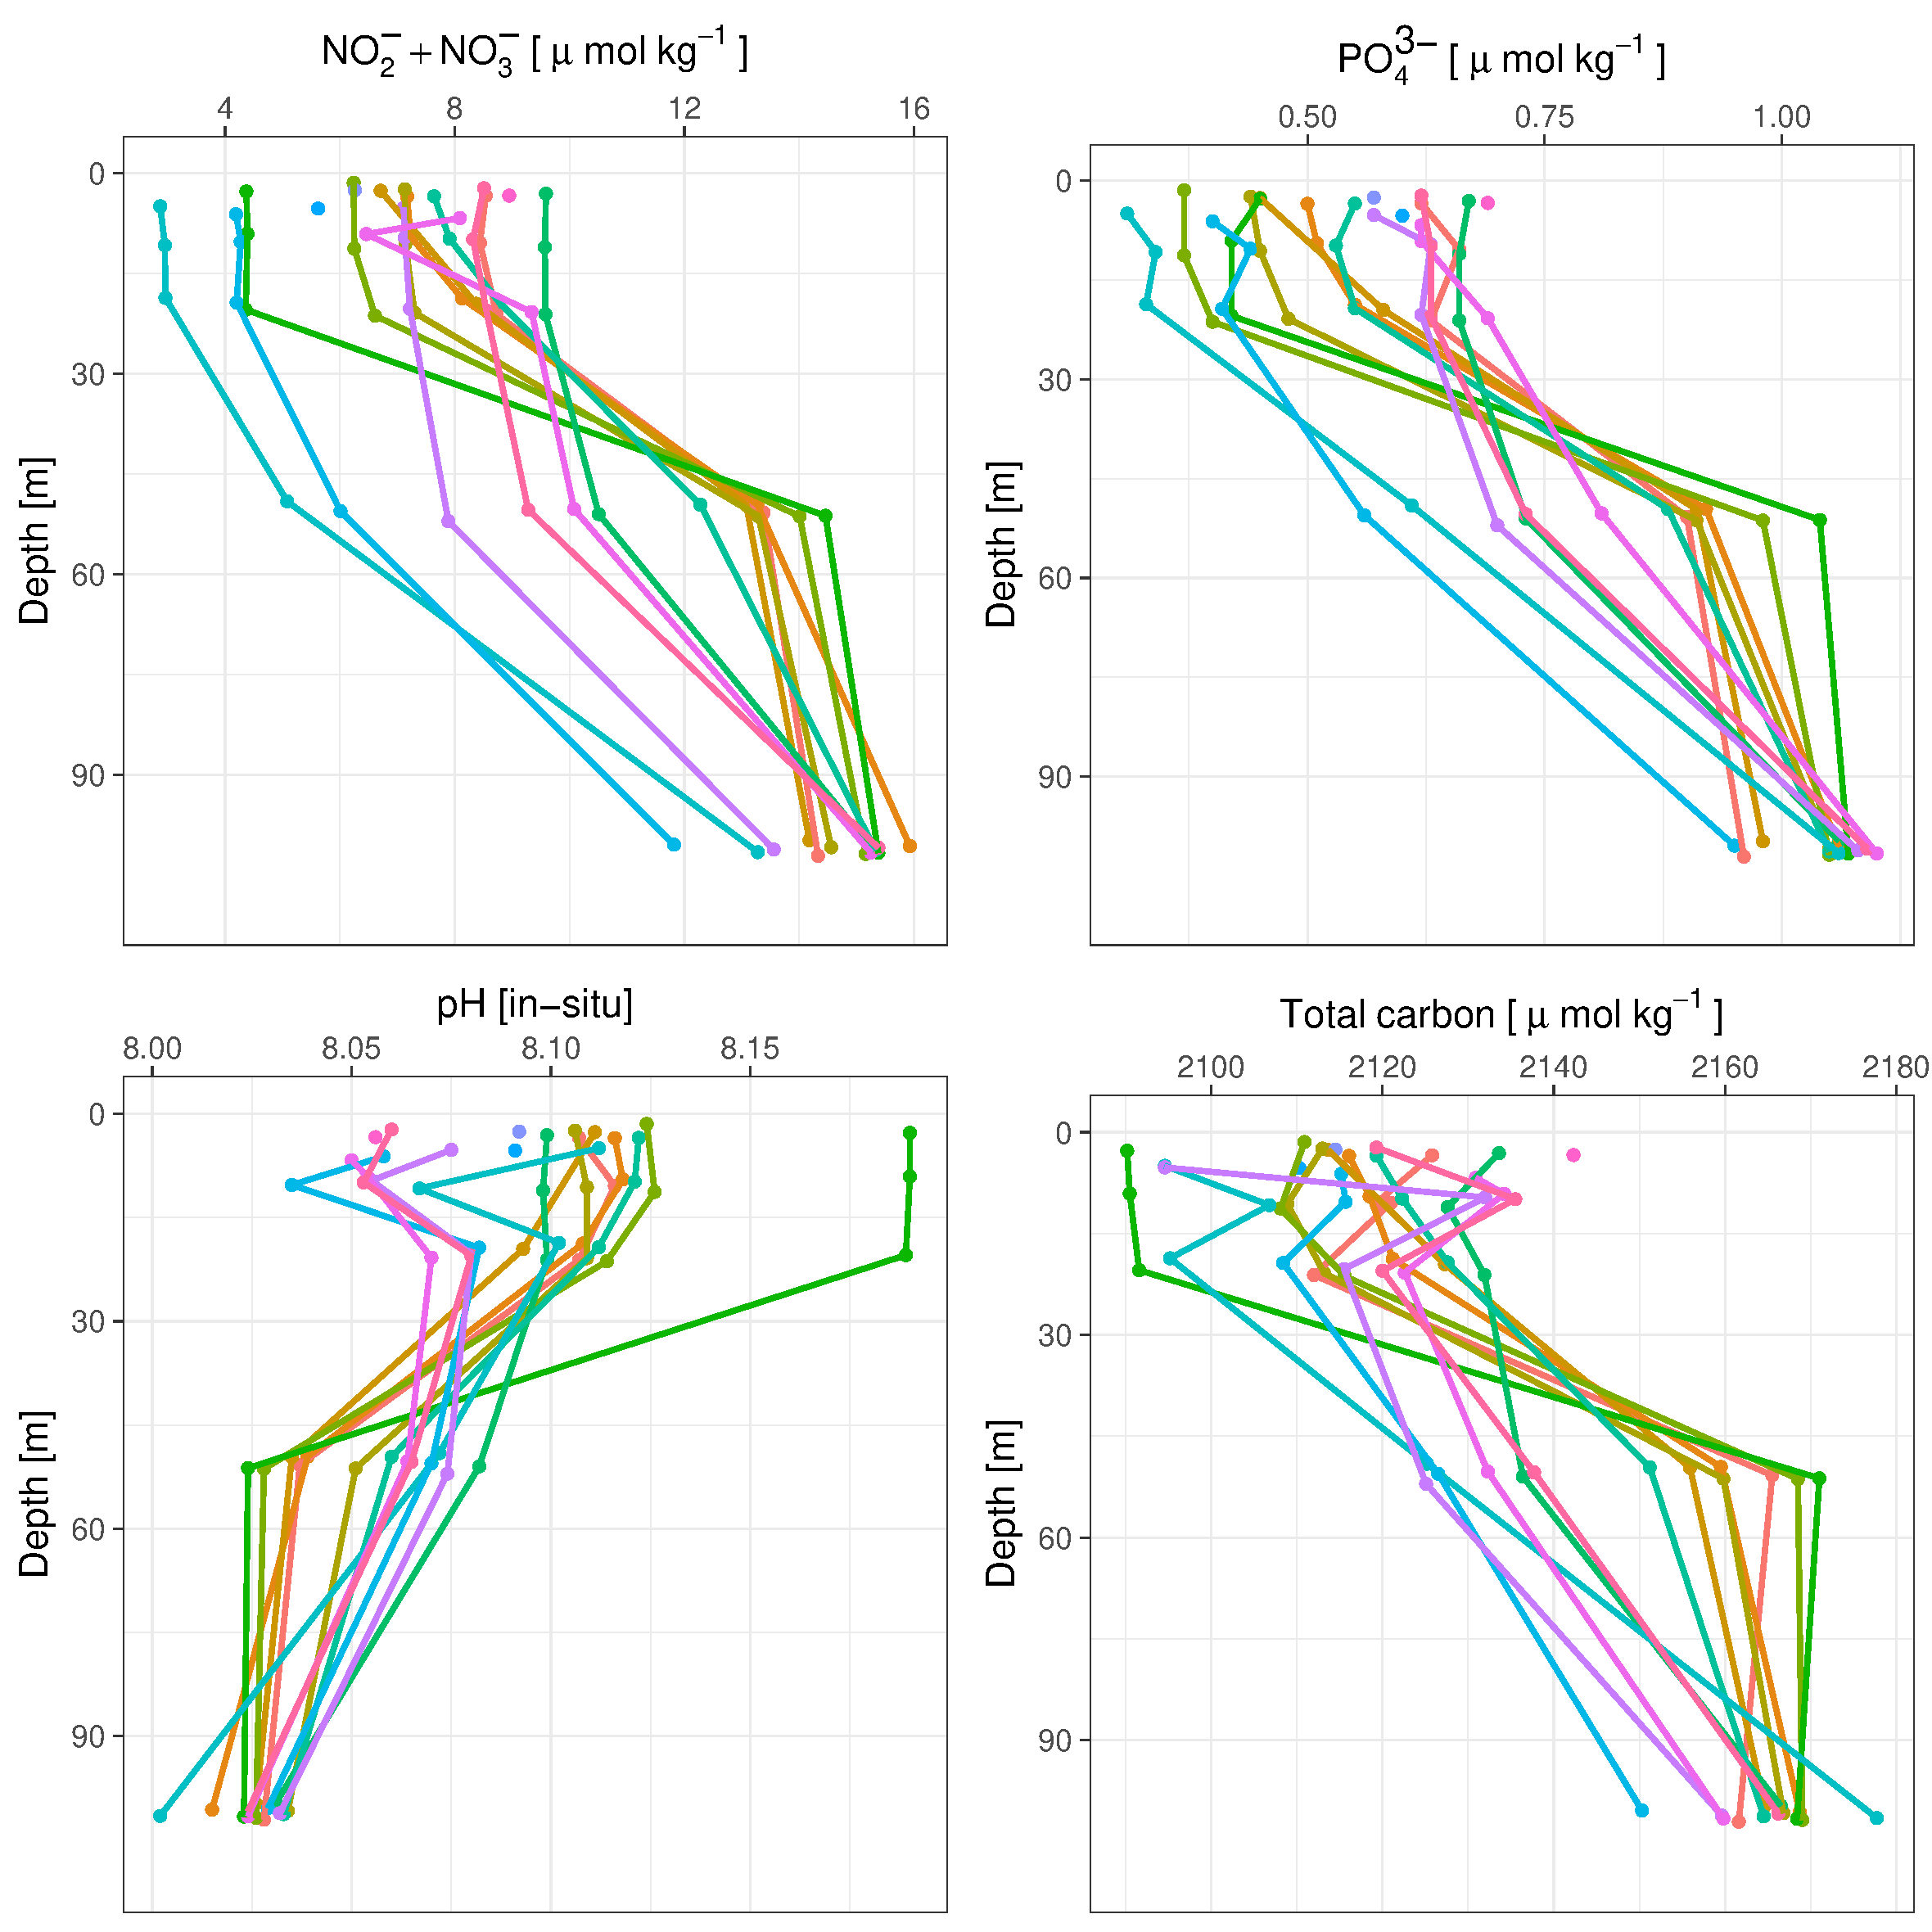
\includegraphics[scale=0.35]{Depth_profiles.pdf} % ask yourself what suffix is being used ...
	\end{center}
	\caption[Field photo of the hydrophone array]{
	\label{f:profile}
	Depth profiles of nitrate, phosphate, pH, and total carbon.}
\end{figure}

\begin{figure}[htbp]
	\begin{center}
		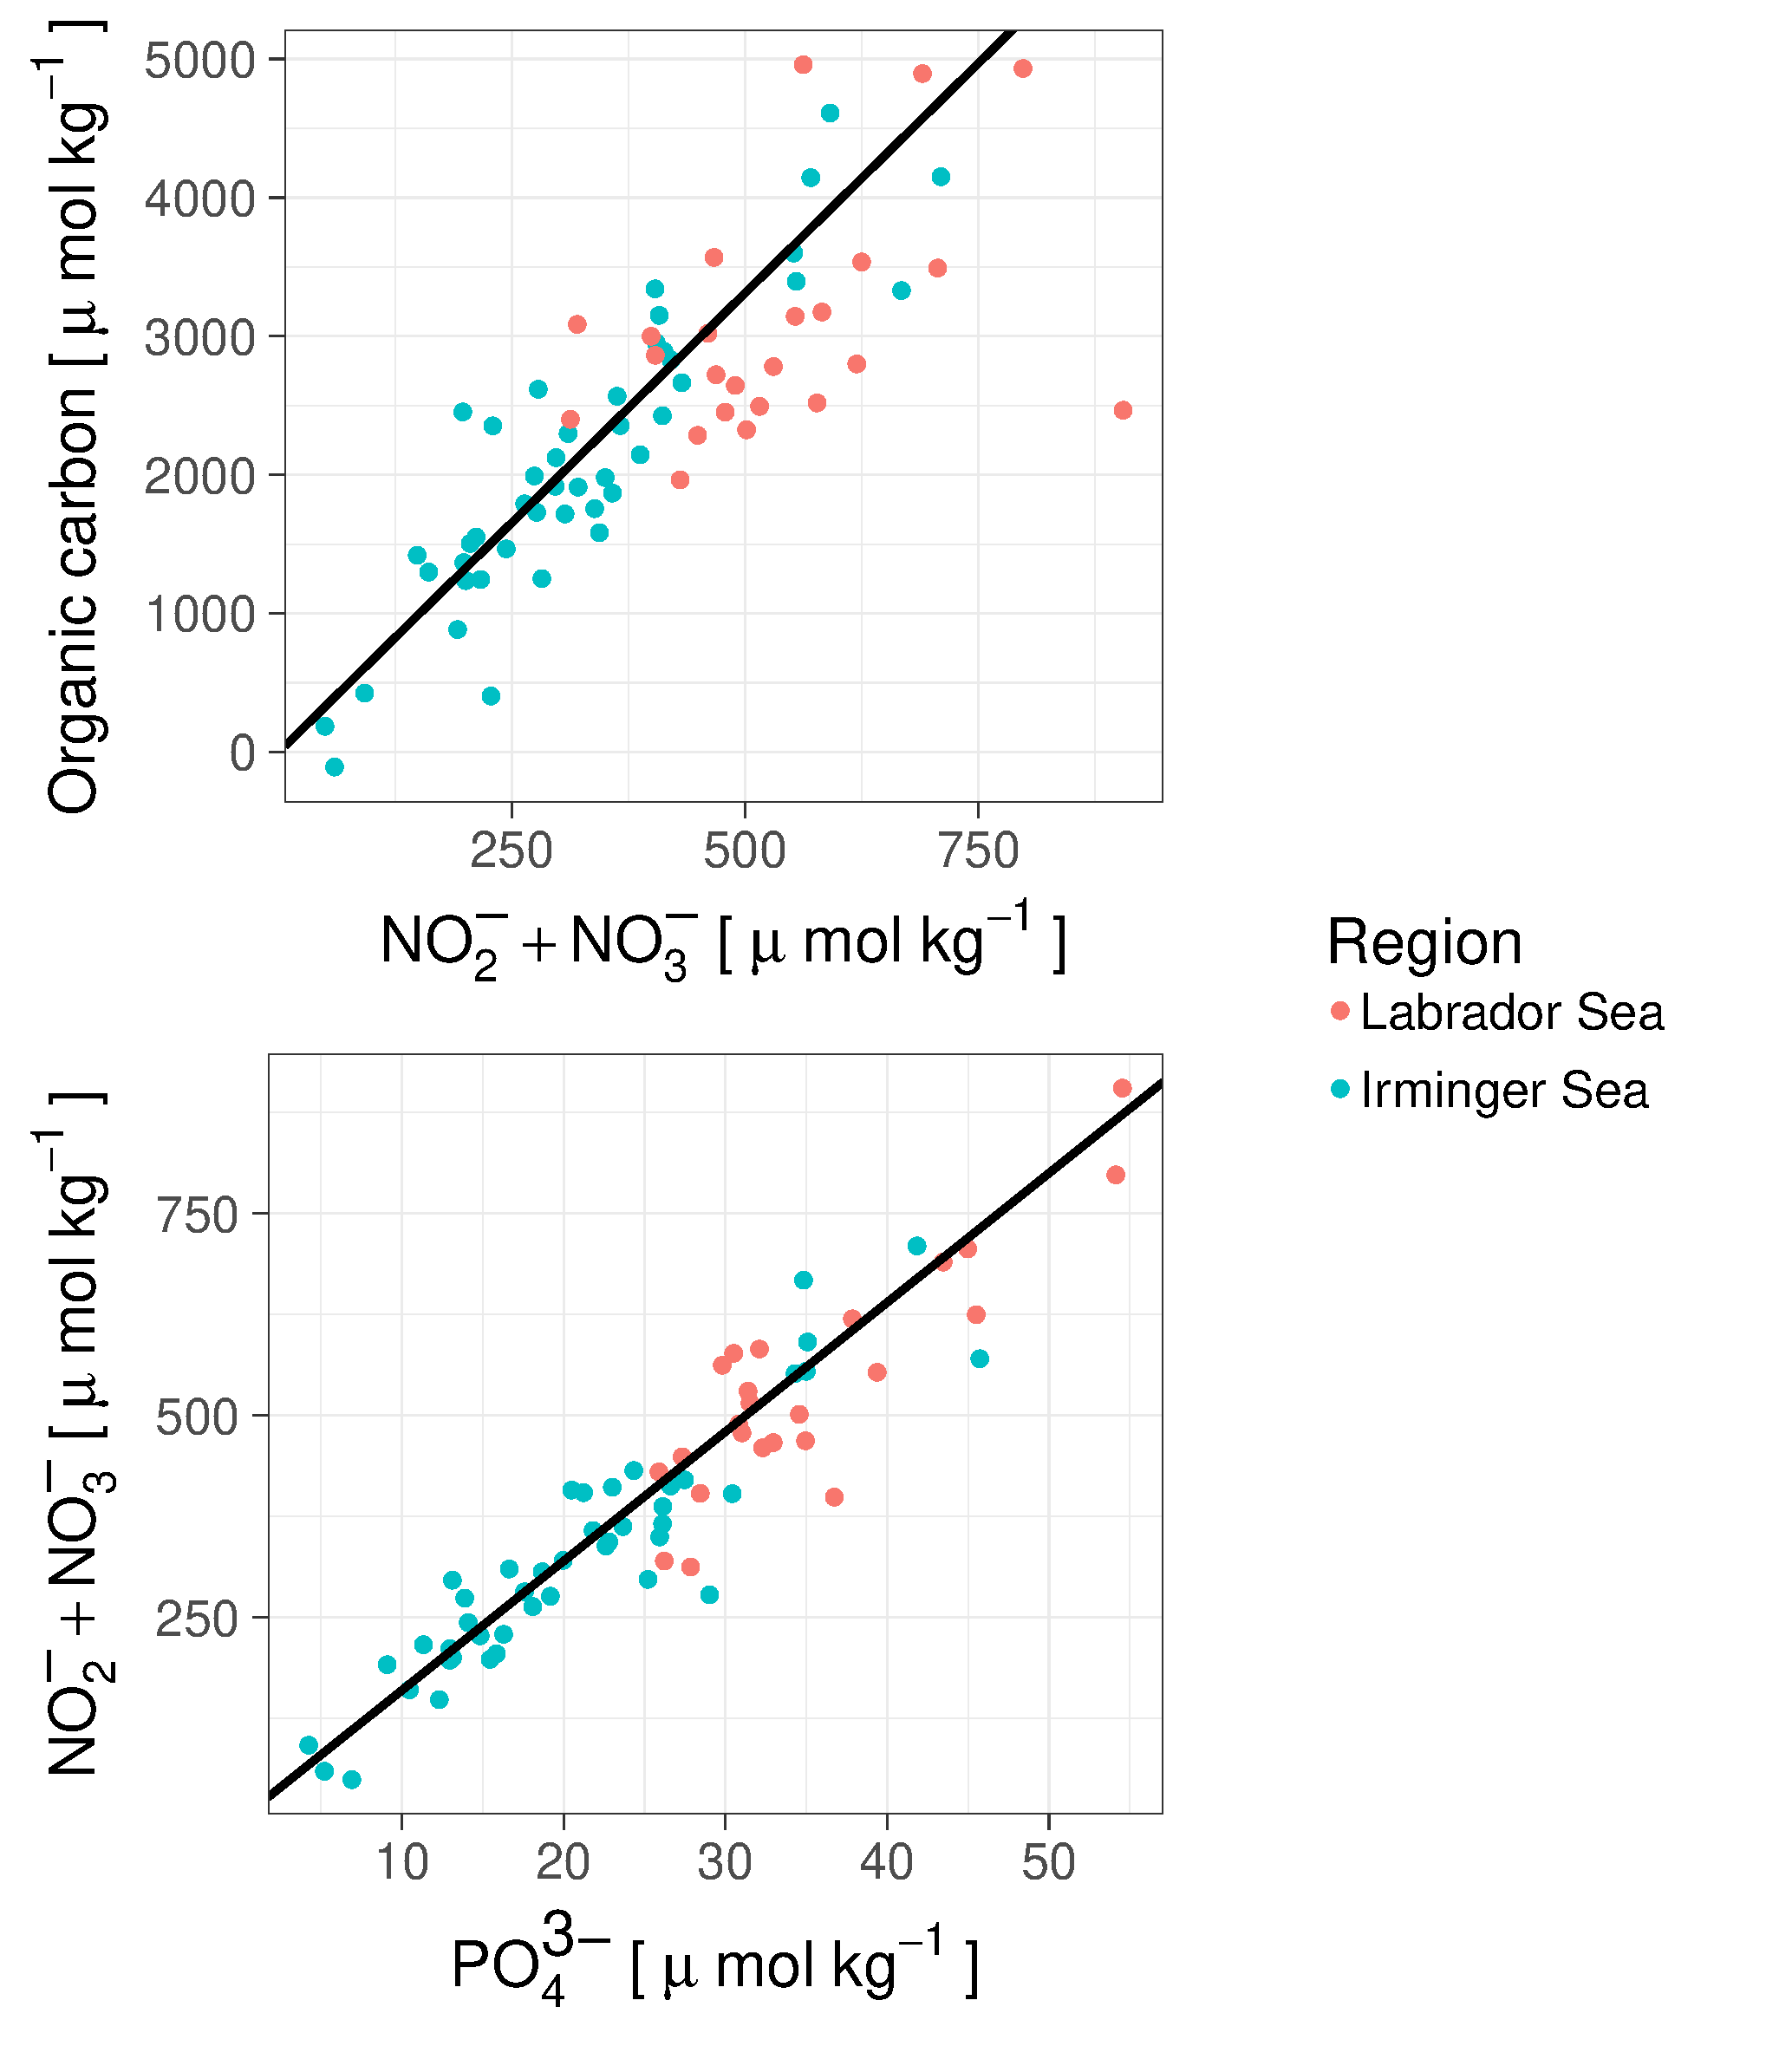
\includegraphics[scale=0.4]{Redfield_comparison.pdf} % ask yourself what suffix is being used ...
	\end{center}
	\caption[Field photo of the hydrophone array]{
	\label{f:redfield}
	Depth profiles of nitrate, phosphate, pH, and total carbon.}
\end{figure}

\begin{figure}[htbp]
	\begin{center}
		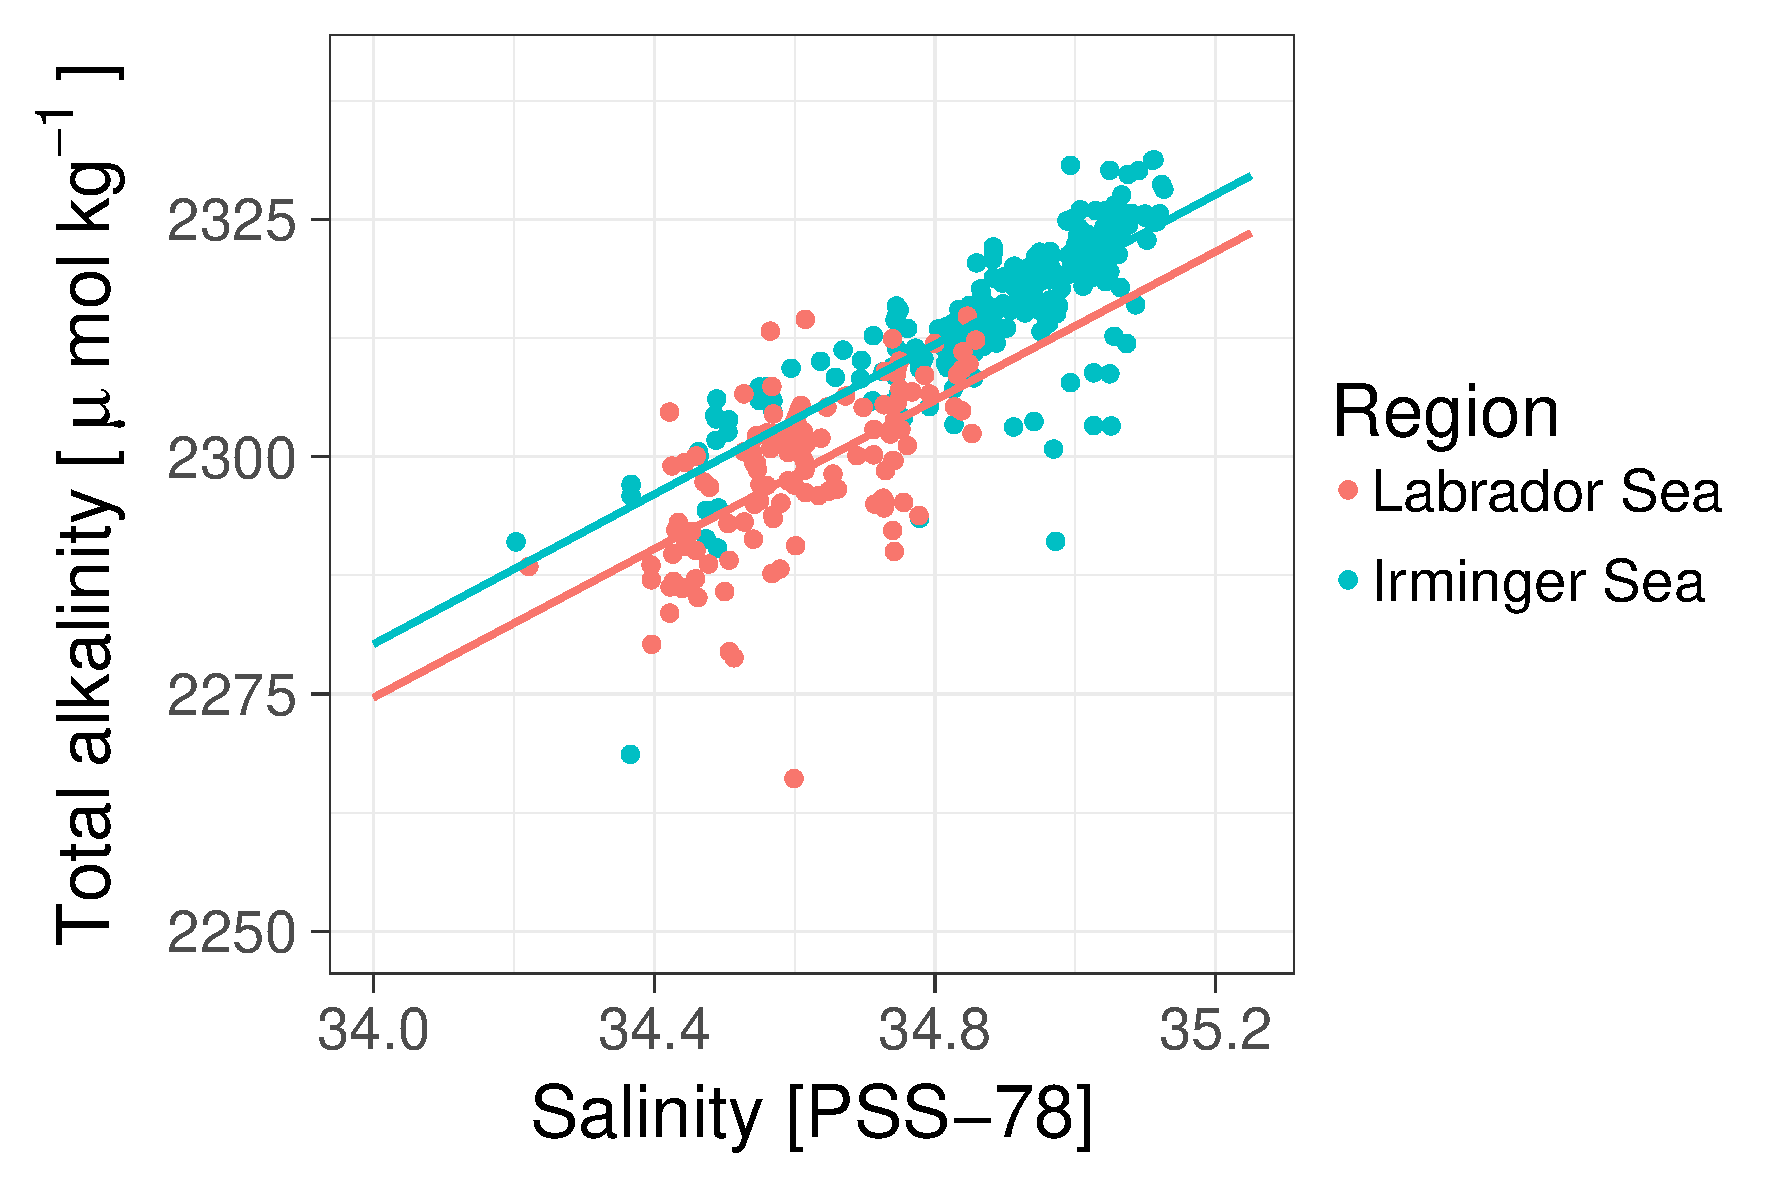
\includegraphics[scale=0.4]{alk_sal.pdf} % ask yourself what suffix is being used ...
	\end{center}
	\caption[Field photo of the hydrophone array]{
	\label{f:array}
	Alkalinity vs. salinity. }
\end{figure}

%\begin{figure}[htbp]
%	\begin{center}
%		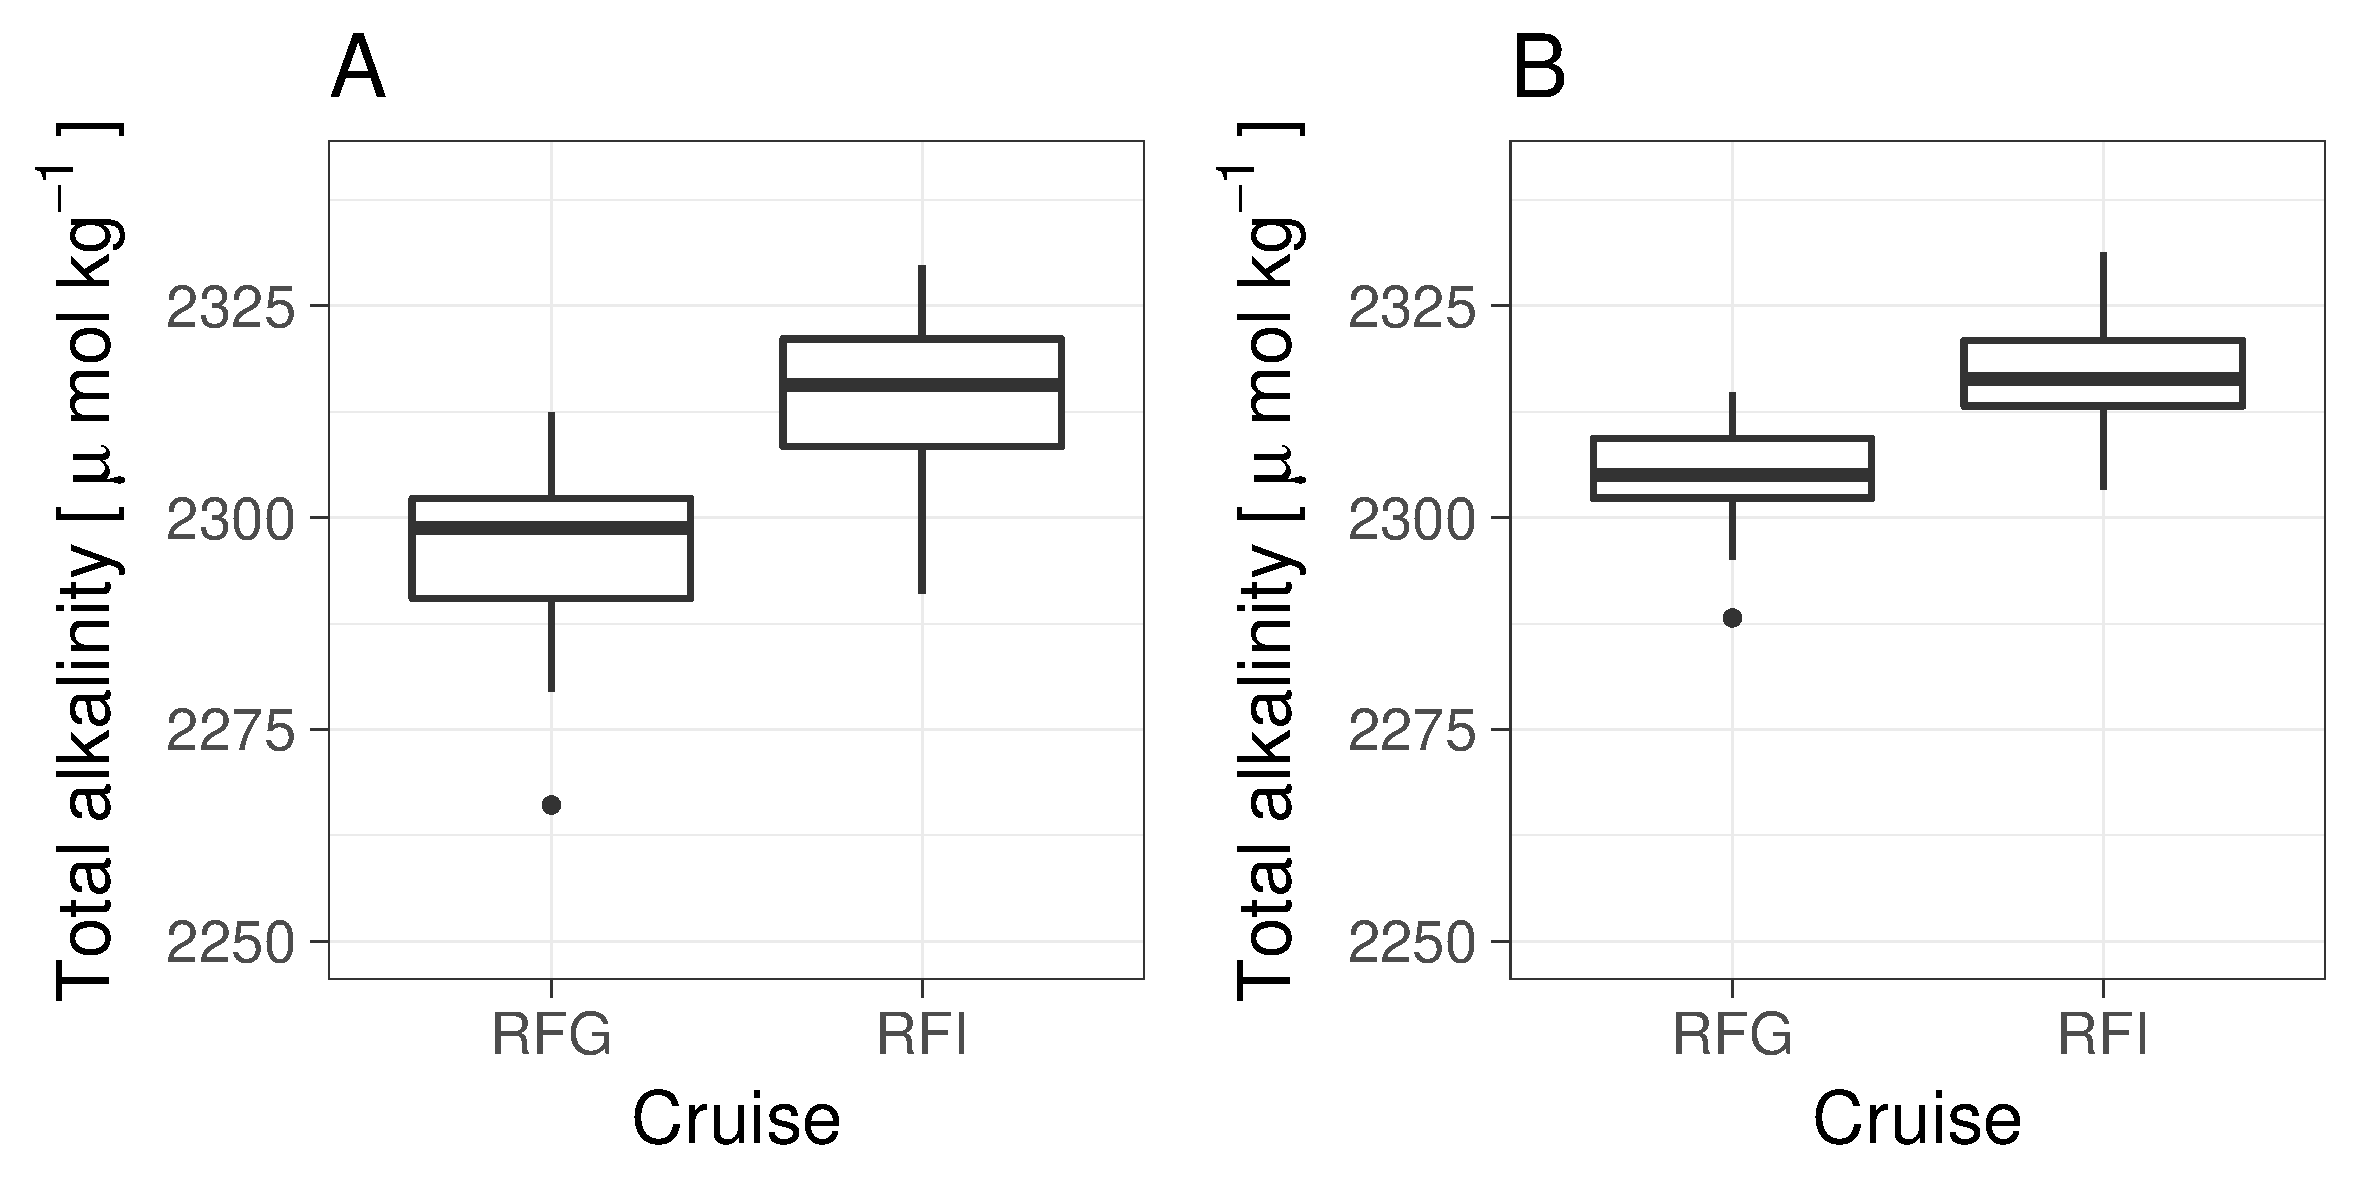
\includegraphics[scale=0.35]{box_alk.pdf} % ask yourself what suffix is being used ...
%	\end{center}
%	\caption[Field photo of the hydrophone array]{
%	\label{f:array}
%	Depth profiles of nitrate, phosphate, pH, and total carbon.}
%\end{figure}
%
%\begin{figure}[htbp]
%	\begin{center}
%		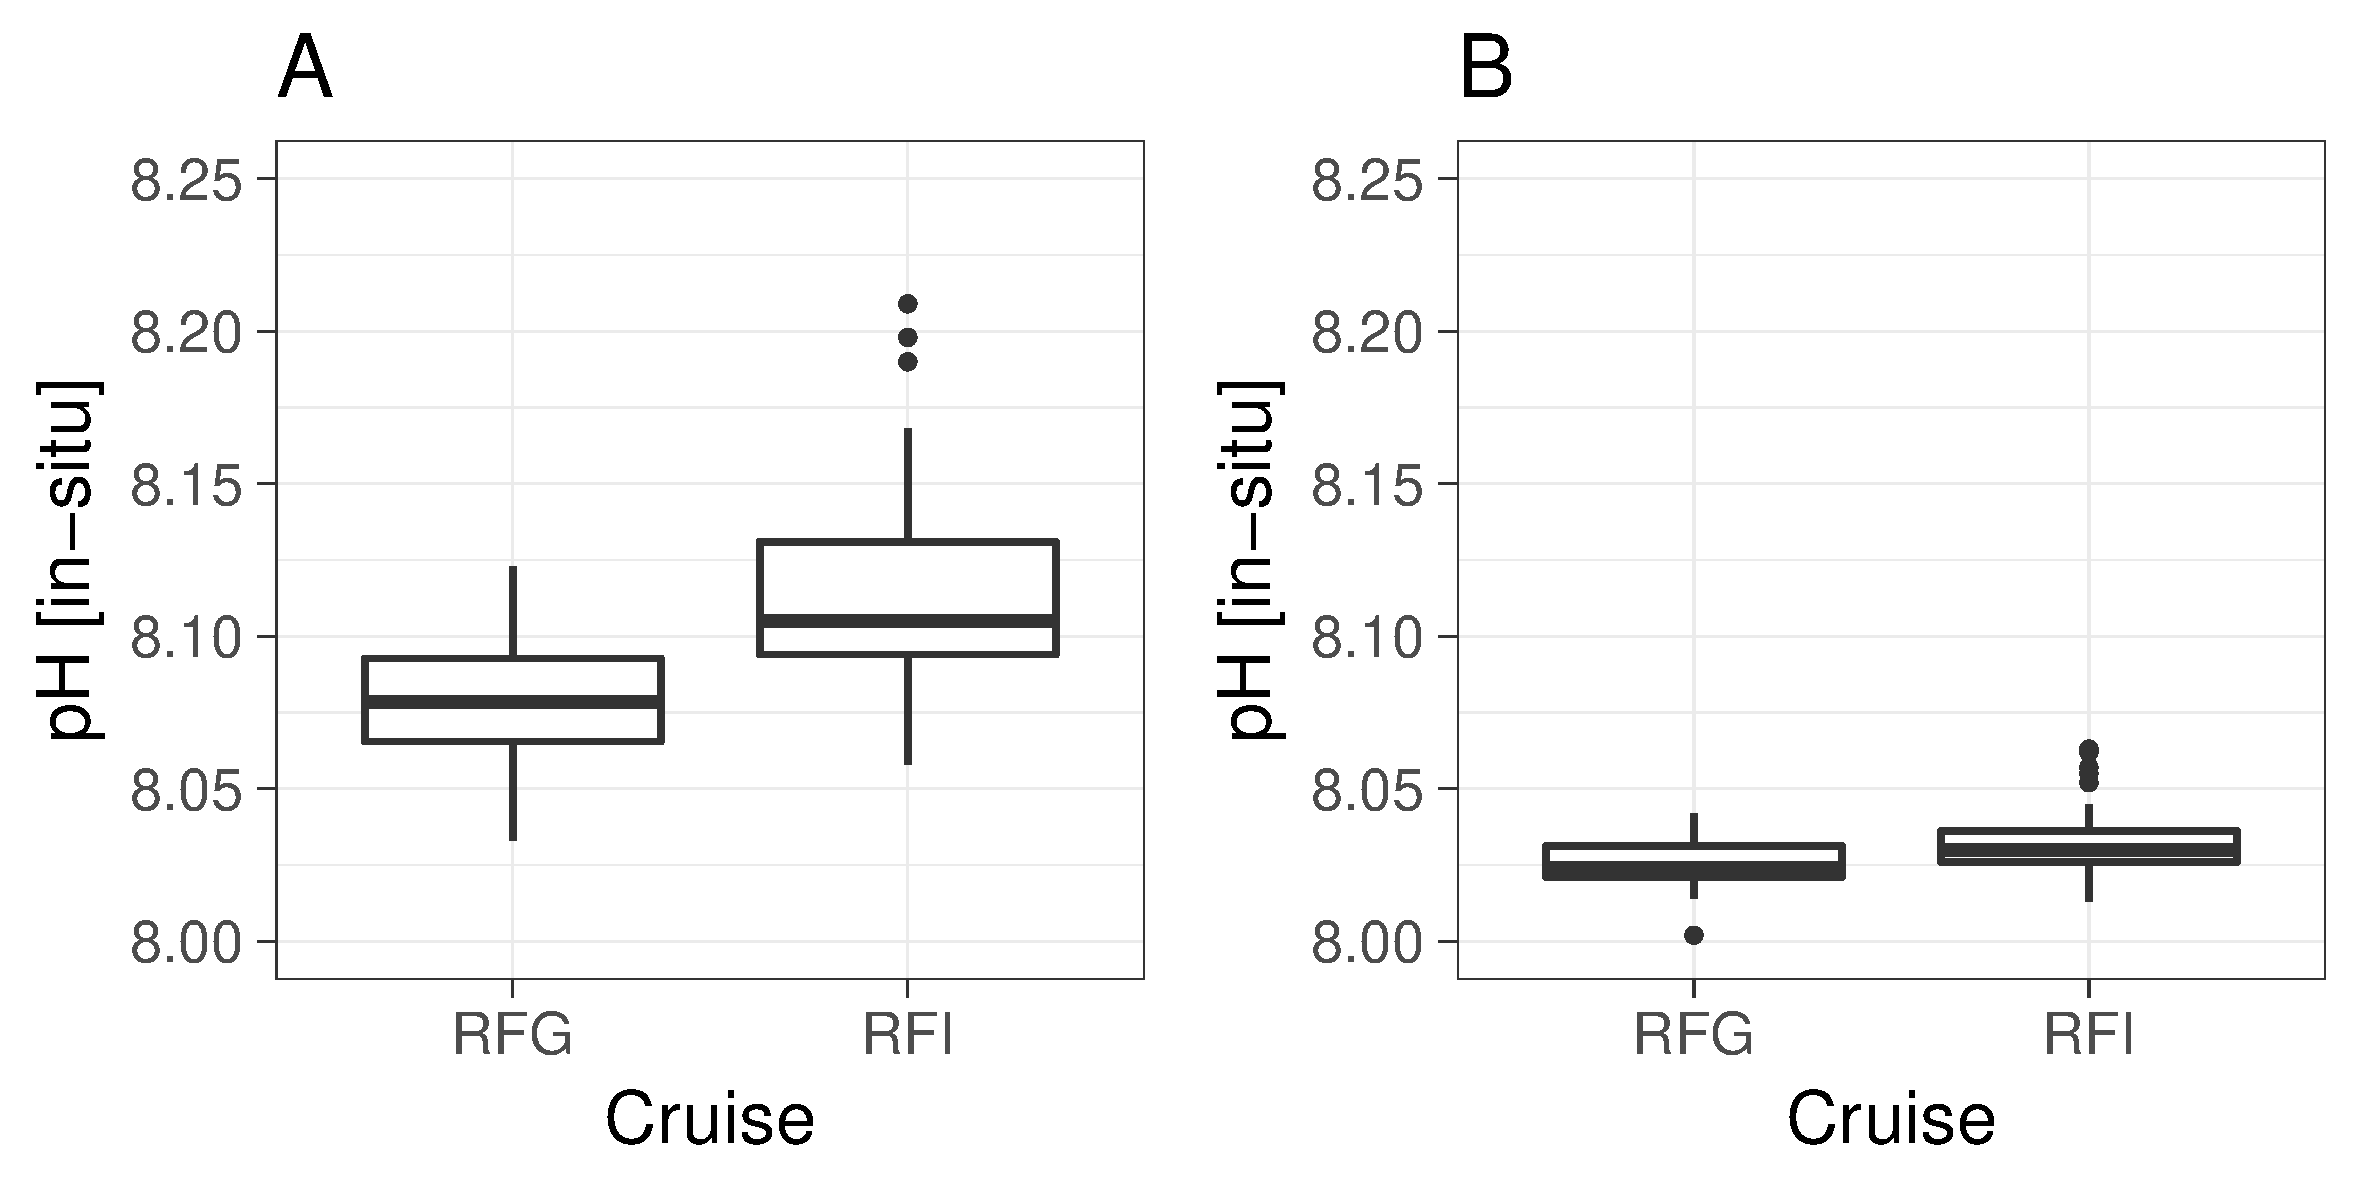
\includegraphics[scale=0.35]{box_ph.pdf} % ask yourself what suffix is being used ...
%	\end{center}
%	\caption[Field photo of the hydrophone array]{
%	\label{f:array}
%	Depth profiles of nitrate, phosphate, pH, and total carbon.}
%\end{figure}
%
%\begin{figure}[htbp]
%	\begin{center}
%		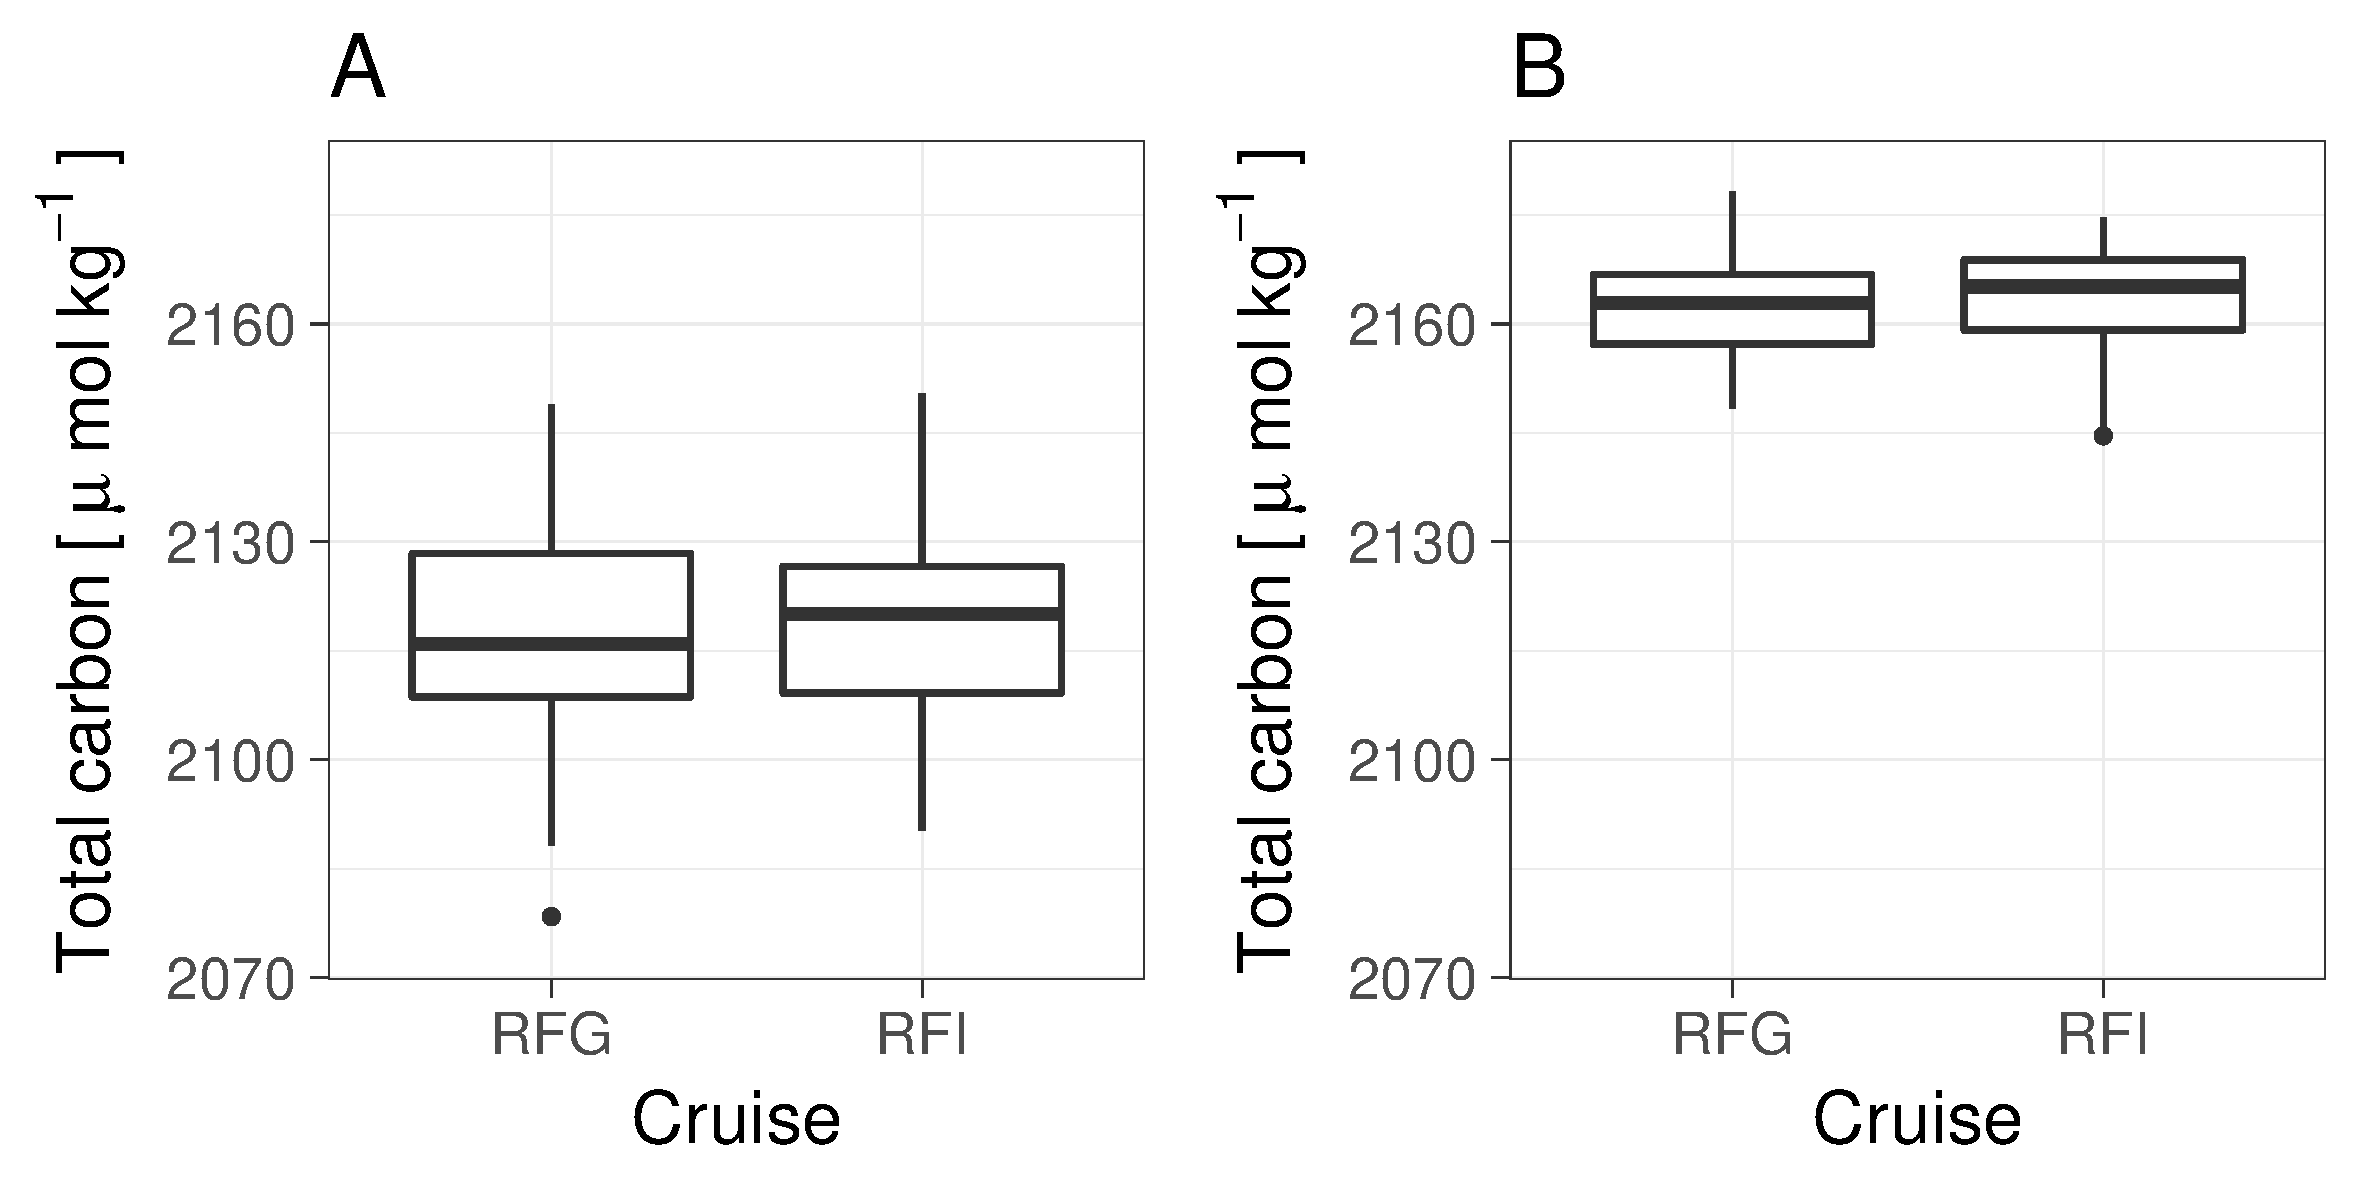
\includegraphics[scale=0.35]{box_C.pdf} % ask yourself what suffix is being used ...
%	\end{center}
%	\caption[Field photo of the hydrophone array]{
%	\label{f:array}
%	Depth profiles of nitrate, phosphate, pH, and total carbon.}
%\end{figure}
%\begin{figure}[htbp]
%	\begin{center}
%		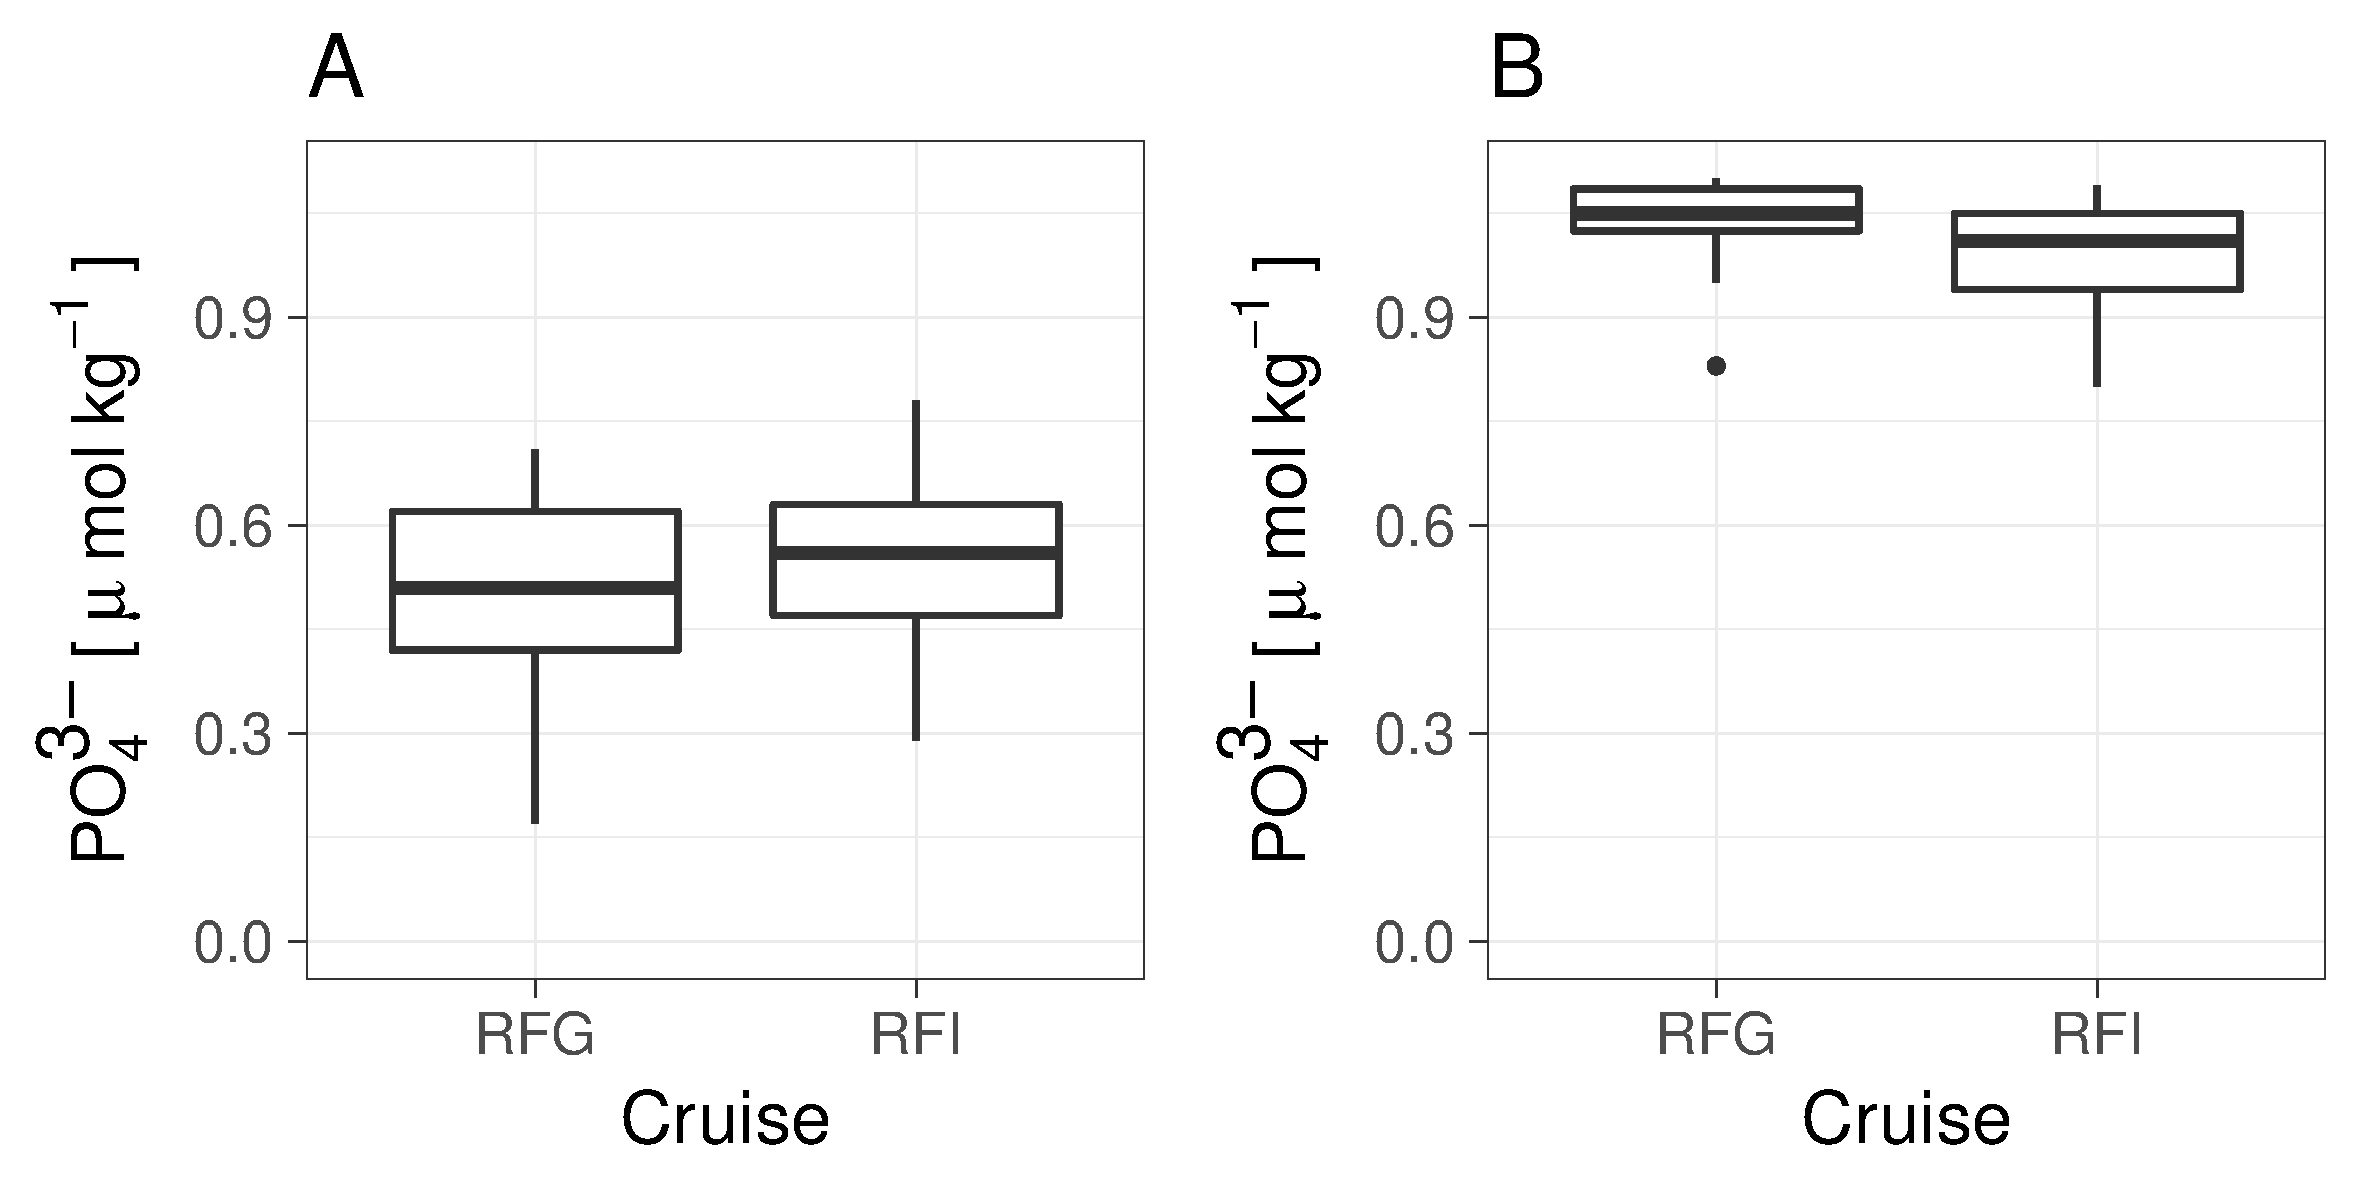
\includegraphics[scale=0.35]{box_P.pdf} % ask yourself what suffix is being used ...
%	\end{center}
%	\caption[Field photo of the hydrophone array]{
%	\label{f:array}
%	Depth profiles of nitrate, phosphate, pH, and total carbon.}
%\end{figure}
%\begin{figure}[htbp]
%	\begin{center}
%		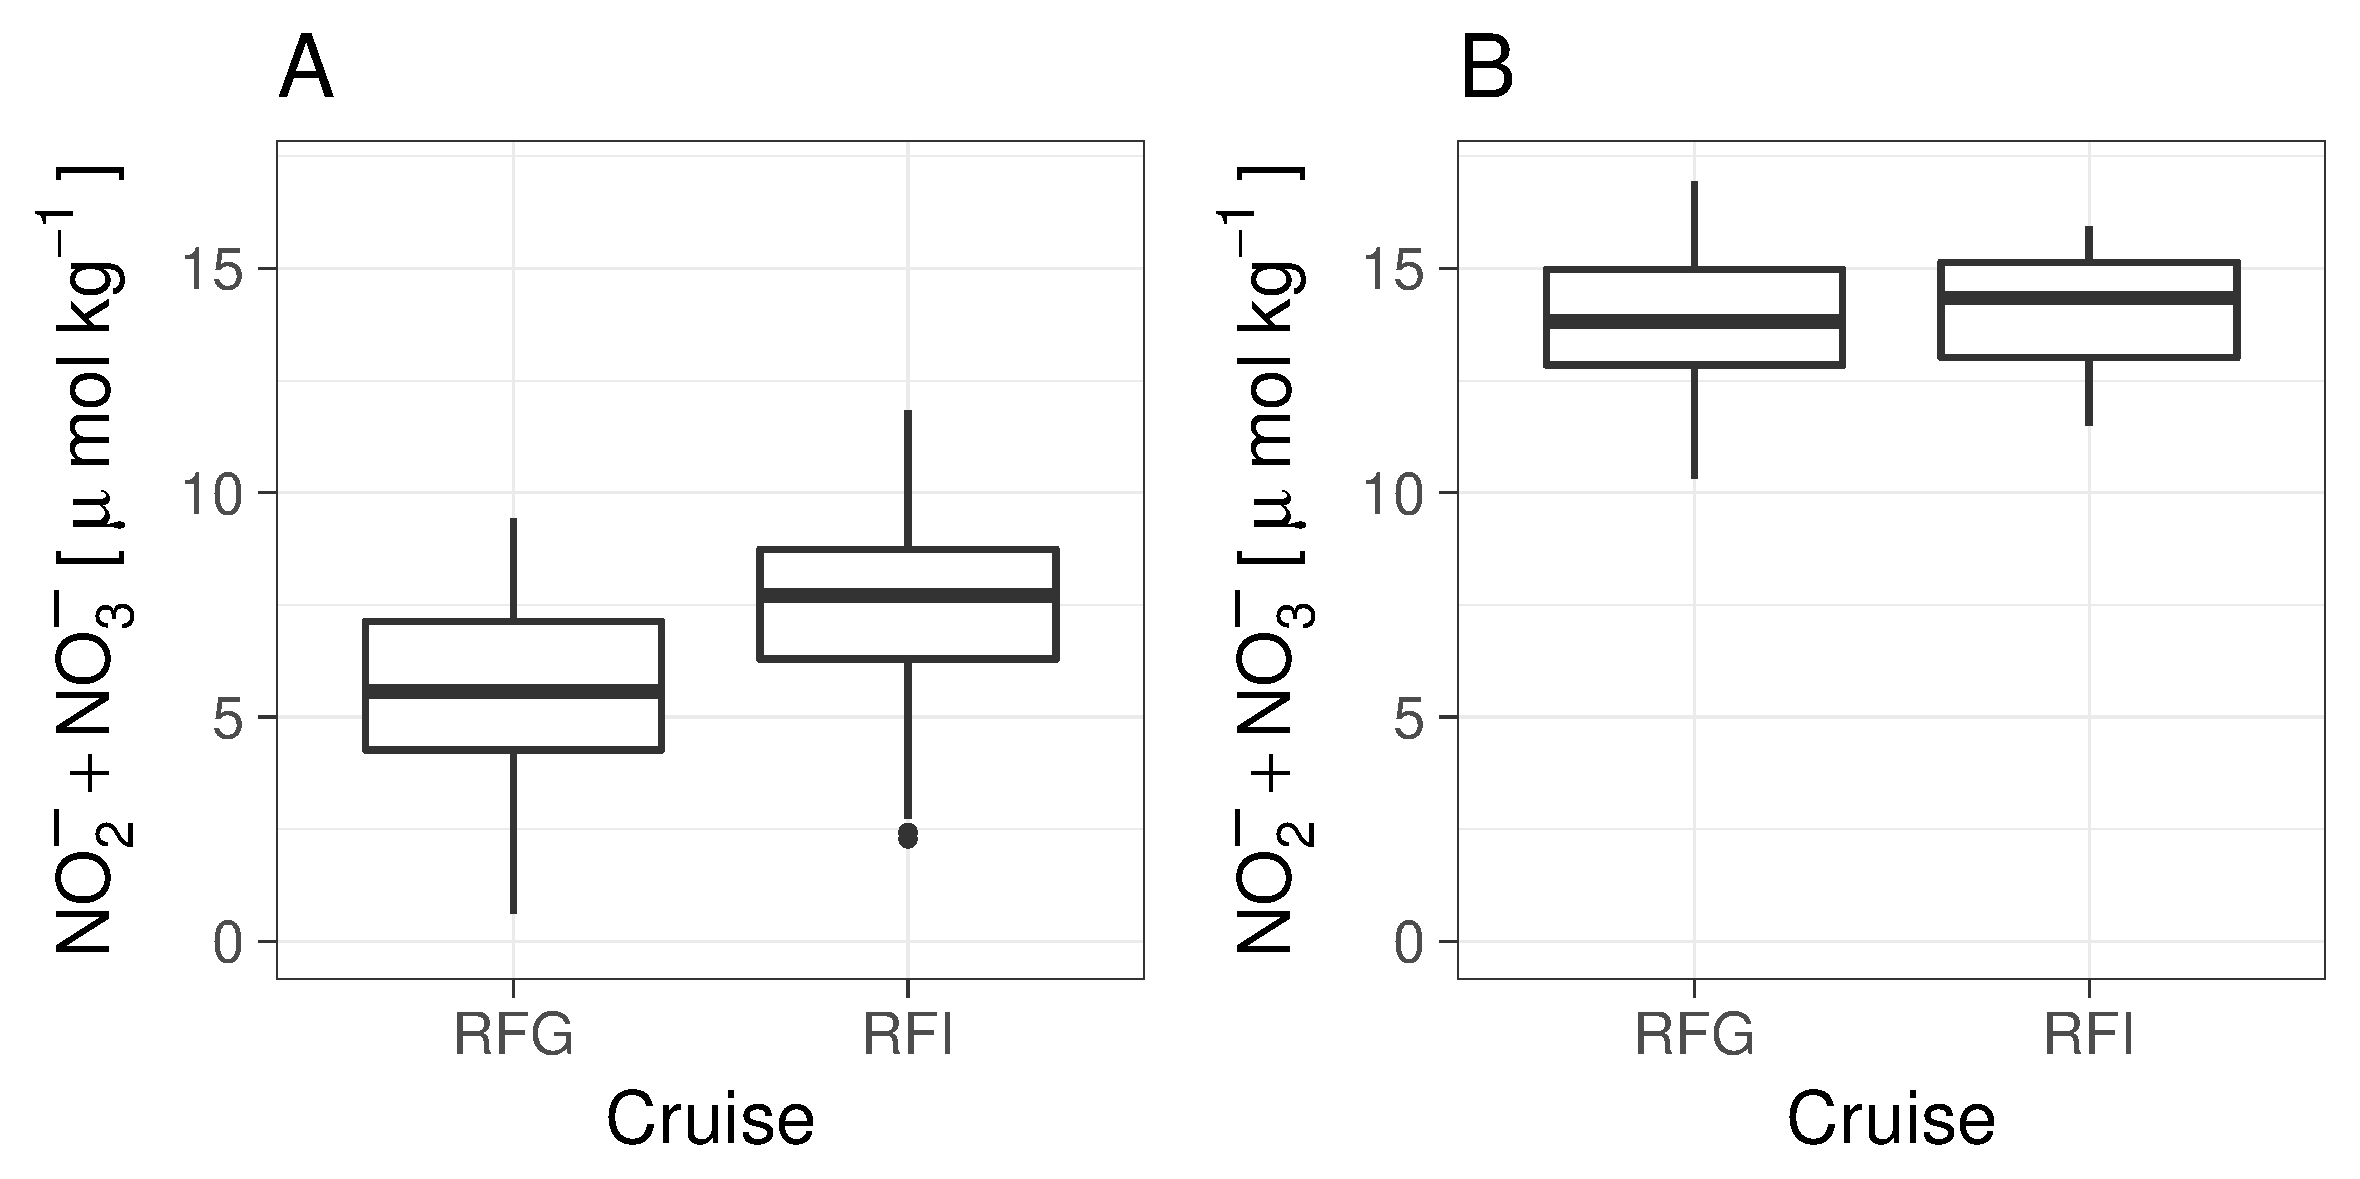
\includegraphics[scale=0.35]{box_N.pdf} % ask yourself what suffix is being used ...
%	\end{center}
%	\caption[Field photo of the hydrophone array]{
%	\label{f:array}
%	Depth profiles of nitrate, phosphate, pH, and total carbon.}
%\end{figure}





















\section{Appendix}



\begin{table}[H] \centering 
  \caption{Sources for the RFI data in the master spreadsheet. \textbf{A:} \protect\path{/redfish_project/old_barkhouse_files/Redfish 2013/2013_pared_down_raw_data.csv}, \textbf{C:} \protect\path{/redfish_project/old_barkhouse_files/Redfish 2013/Dan_Kelly_Data.xlsx}, \textbf{D:} \protect\path{/redfish_project/old_barkhouse_files/Redfish 2013/CARINA/CARINA_COMBINED.xlsx}}
  \label{t:RFIsources} 
\begin{tabular}{p{3cm}p{10cm}}%{@{\extracolsep{5pt}} ll}
\\[-1.8ex]\hline 
\hline \\[-1.8ex] 
 Variable & Source\\ 
\hline \\[-1.8ex] 
Expocode & Unknown\\[8pt] 
Section number & Unknown\\[8pt] 
Station number & A\\[8pt] 
Cast number & Unknown\\[8pt] 
Bottle number & Unknown\\[8pt] 
Time & Unknown\\[8pt] 
Date & Unknown\\[8pt] 
Latitude & Unknown\\[8pt] 
Longitude  & Unknown\\[8pt] 
Depth  & Unknown\\[8pt] 
CTD Pressure & A\\[8pt] 
CTD Temperature & A\\[8pt] 
Conductivity  & N/A\\[8pt] 
Salinity & A\\[8pt] 
Total Alkalinity & A\\[8pt] 
pH & A\\[8pt] 
Total Carbon & A\\[8pt] 
pCO2 & C + D\\[8pt] 
NO2+NO3 & A\\[8pt] 
PO4 & A\\[8pt] 
SiO2 & A\\[8pt] 
?ar & A\\[8pt] 
\hline \\[-1.8ex]
\end{tabular} 
\end{table} 

\begin{table}[H] \centering 
  \caption{Sources for the RFG data in the master spreadsheet. \textbf{B:} \protect\path{/redfish_project/old_barkhouse_files/Redfish 2013/German_Redfield/German_redfield.csv}}
  \label{t:RFGsources} 
\begin{tabular}{p{3cm}p{10cm}}%{@{\extracolsep{5pt}} ll}
\\[-1.8ex]\hline 
\hline \\[-1.8ex] 
 Variable & Source\\ 
\hline \\[-1.8ex] 
Expocode & B\\[8pt] 
Section number & B\\[8pt] 
Station number & B\\[8pt] 
Cast number & B\\[8pt] 
Bottle number & B\\[8pt] 
Time & Unknown\\[8pt] 
Date & B\\[8pt] 
Latitude & B\\[8pt] 
Longitude  & B\\[8pt] 
Depth  & B\\[8pt] 
CTD Pressure & B\\[8pt] 
CTD Temperature & B\\[8pt] 
Conductivity  & B\\[8pt] 
Salinity & B\\[8pt] 
Total Alkalinity & B\\[8pt] 
pH & B\\[8pt] 
Total Carbon & B\\[8pt] 
pCO2 & B\\[8pt] 
NO2+NO3 & B\\[8pt] 
PO4 & B\\[8pt] 
SiO2 & B\\[8pt] 
?ar & B\\[8pt] 
\hline \\[-1.8ex]
\end{tabular} 
\end{table} 

\begin{table}[H] \centering
  \caption{Parameter ranges at the surface and at 100m in the water column.}
  \label{t:Ranges} 
\begin{tabular}{llrrl}
  \\[-1.8ex]\hline 
\hline \\[-1.8ex] 
 Measurement & Depth & Minimum value & Maximum value & Units\\ 
\hline \\[-1.8ex] 
Alkalinity & Surface & 2194.02 & 2329.74 & $\mu$ mol kg$^{-1}$\\ 
pH & Surface & 8.03 & 8.21& in-situ\\ 
Total carbon & Surface & 2013.40 & 2150.40 &$\mu$ mol kg$^{-1}$\\ 
\ce{pCO2} & Surface & 241.00 & 400.70& $\mu$atm\\ 
\ce{NO2^-} + \ce{NO3^-} & Surface & 0.62 & 11.84& $\mu$ mol kg$^{-1}$\\ 
\ce{PO4^{3-}} & Surface & 0.17 & 0.78&$\mu$ mol kg$^{-1}$ \\ 
Si & Surface & 0.02 & 9.34& $\mu$ mol kg$^{-1}$\\ 
\hline \\[-1.8ex] 
Alkalinity & 100 m & 2288.17 & 2331.28& $\mu$ mol kg$^{-1}$\\ 
pH & 100 m & 7.97 & 8.06& in-situ\\ 
Total carbon & 100 m & 2144.60 & 2178.30&$\mu$ mol kg$^{-1}$ \\ 
\ce{pCO2}  & 100 m & 367.80 & 462.30& $\mu$atm\\ 
\ce{NO2^-} + \ce{NO3^-} & 100 m & 10.32 & 16.95 &$\mu$ mol kg$^{-1}$\\ 
\ce{PO4^{3-}}  & 100 m & 0.80 & 1.24 &$\mu$ mol kg$^{-1}$\\ 
 Si & 100 m & 3.96 & 12.05 &$\mu$ mol kg$^{-1}$\\ 
   \hline
\end{tabular}
\end{table}

\begin{table}[H] \centering
  \caption{Nutrient ratio statistics from Irminger Sea measurements.}
  \label{t:RFI} 
\begin{tabular}{llrrl}
  \\[-1.8ex]\hline 
\hline \\[-1.8ex] 
 Nutrient ratio & Mean & Median & Standard deviation \\ 
\hline \\[-1.8ex] 
C:N & 6.38 & 6.44 & 2.16 \\ 
C:P & 100.07 & 98.97 & 34.38 \\ 
N:P & 15.71 & 15.33 & 3.06 \\ 
   \hline
\end{tabular}
\end{table}


\begin{table}[H] \centering
  \caption{Nutrient ratio statistics from Labrador Sea measurements.}
  \label{t:RFG} 
\begin{tabular}{llrrl}
  \\[-1.8ex]\hline 
\hline \\[-1.8ex] 
Nutrient ratio & Mean & Median & Standard deviation \\ 
\hline \\[-1.8ex] 
C:N & 5.93 & 5.55 & 1.57 \\ 
C:P & 88.80 & 83.09 & 22.45 \\ 
N:P & 15.23 & 15.57 & 2.11 \\ 
   \hline
\end{tabular}
\end{table}

\begin{table}[H] \centering
  \caption{Nutrient ratio statistics from all of the Redfish 2013 data.}
  \label{t:Broad} 
\begin{tabular}{llrrl}
  \\[-1.8ex]\hline 
\hline \\[-1.8ex] 
Nutrient ratio & Mean & Median & Standard deviation \\ 
\hline \\[-1.8ex] 
C:N & 6.22 & 6.17 & 1.97 \\ 
C:P & 96.15 & 94.15 & 31.06 \\ 
N:P & 15.54 & 15.43 & 2.76 \\ 
   \hline
\end{tabular}
\end{table}

%\end{multicols}
\end{document}
